\newpage
\section{Durchführung}
\subsection{Pockels-Effekt}
\begin{figure}[h]
\begin{center}
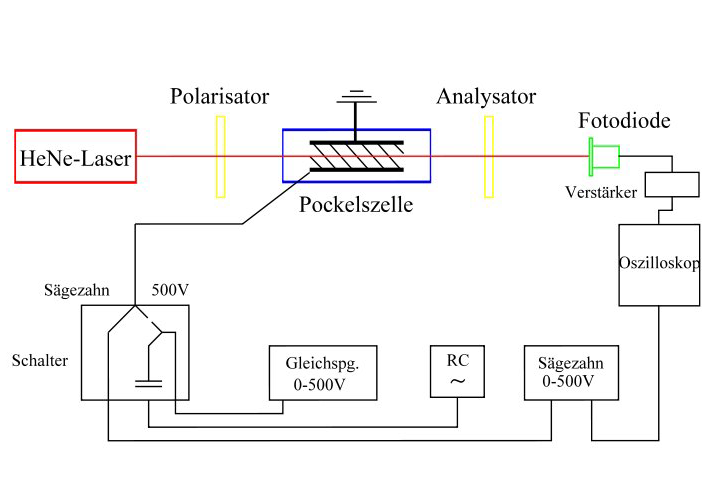
\includegraphics[scale=0.5]{durchpock.png}
\caption{Aufbau}
\end{center}
\end{figure}
Der Aufbau besteht aus einem He-Ne-Laser als Lichtquelle, welche ihren Strahl durch einen Polarisator sendet, der dafür sorgt, dass das Licht linear polarisiert ist. Nach diesem Vorgang trifft der Strahl auf die Pockels-Zelle, in welcher die Richtung der Polarisation verändert wird. Zunächst ist dieser Aufbau zu justieren. Ein Analysator wird verwendet, um die Intensität abhängig von dem Winkel relativ zur Polarisationsrichtung zu verändern. Das Licht wird schließlich von einer Photodiode mit einem Verstärker detektiert. Das nachgeschaltete Oszilloskop stellt den Verlauf des resultierenden Signals dar. Es kann auch das Eingangssignal anzeigen. Die unterschiedlichen Spannungsverläufe werden von einem Spannungsgenerator geliefert. Die auf dem Oszilloskop dargestellten Signale können mithilfe eines Computerprogramms ausgelesen werden. Es ist darauf zu achten, dass die Auflösung auf dem Oszilloskop möglich groß ist und die Signale komplett auf den Bildschirm passen. Damit nehmen wir dann mithilfe des PC-Programmes den Kurvenverlauf auf und schließlich auch ein gedämpftes und ein ungedämpftes Signal. Im zweiten Teil des Versuchs (für den Sinus-Verlauf) muss am Spannungsgenerator die Spannung verändert werden, bis eine Verdopplung der Frequenz beobachtet wird. Diese Messreihe wird für negative wie positive Spannungen öfters wiederholt.